% This must be in the first 5 lines to tell arXiv to use pdfLaTeX.
\pdfoutput=1
% Lexical complexity prediction for Romanian -- ML course project report.
% Figures live in report/figures/. Compile on Overleaf with the ACL template (acl.sty, acl_natbib.bst).
% References: paste custom.bib, then Recompile twice (pdfLaTeX -> bibtex -> pdfLaTeX).

\documentclass[11pt]{article}

\usepackage[review]{acl}

\usepackage{times}
\usepackage{latexsym}
\usepackage[T1]{fontenc}
\usepackage[utf8]{inputenc}
\usepackage{microtype}
\usepackage{graphicx}
\usepackage{booktabs}

\graphicspath{{figures/}}

% Float placement: let floats fill pages so no near-empty float page is created.
\setcounter{topnumber}{3}
\renewcommand{\topfraction}{0.92}
\renewcommand{\bottomfraction}{0.85}
\renewcommand{\floatpagefraction}{0.85}
\renewcommand{\textfraction}{0.06}

\title{Cross-Lingual Transfer for Romanian Lexical Complexity Prediction:
Fusing a Multilingual Encoder, a Language Model, Surprisal, and Eye-Tracking}

\author{
  Alexandru Cojoaca \\
  {\small\texttt{alexandru.cojoaca@s.unibuc.ro}} \\\And
  Mihai-Alexandru Preoteasa \\
  {\small\texttt{mihai-alexandru.preoteasa@s.unibuc.ro}} }

\begin{document}
\maketitle

\begin{abstract}
This work estimates how difficult a Romanian word is to read, in context, as a score in $[0,1]$. No Romanian data
annotated with complexity is available for training, so no model is trained on Romanian labels; instead, complexity
knowledge is transferred from resources in other languages and from a Romanian language model, and eye-tracking
data is added. The final prediction combines four complementary signals: cross-lingual transfer, a language-model
difficulty rating, surprisal, and an eye-tracking reading-effort score.
\end{abstract}

\section{Introduction}
\label{section:intro}
Lexical complexity prediction means assigning each target word in a sentence a score: common, easy words score low,
rare or hard words score high. The difficulty here is the absence of Romanian data annotated with complexity for
training. The performance metric combines correlation and fit, $50\,(|r| + \max(0,R^2))$.

Instead of training, the approach reuses complexity knowledge that already exists in other resources. The following
approaches were tried:
\begin{itemize}
  \item cross-lingual transfer from English and Romance annotations through a multilingual model, with a frequency
        correction for Romanian inflection;
  \item a difficulty rating and a surprisal signal from the RoLlama3-8B language model;
  \item a reading-effort signal derived from the eye-tracking measurements through principal component analysis;
  \item approaches that did not help: fine-tuning, encoder swaps, chain-of-thought and few-shot prompting, and
        additional lexical features.
\end{itemize}

% TODO: author contributions.
Two ideas shaped the design: combining contextual embeddings with simple lexical features, and treating frequency
as central while keeping complexity distinct from difficulty. The signals also rest on surprisal theory
\citep{hale2001probabilistic}, recently confirmed against eye-tracking in a Romance language
\citep{gaze4nlp2025surprisal}, and the model is interpreted with SHAP \citep{lundberg2017shap}.

\section{Approach}
\label{section:approach}

\subsection{Setup and validation}
The system uses XLM-RoBERTa-base and RoLlama3-8B (4-bit quantized), with \texttt{transformers},
\texttt{scikit-learn} and \texttt{wordfreq}.
Because no Romanian complexity labels are available for training, validation is done in-source instead: a regressor
is trained on one set of languages and tested on another, with cross-validation within each source. Built on
thousands of real labels, the in-source check indicates whether a configuration is sound before transfer to
Romanian. A recurring lesson (Section~\ref{sec:negative}) is that a good in-source number does not guarantee a good
Romanian result.

\subsection{The four signals}
Each signal estimates complexity in a different way.

\textbf{(A) Cross-lingual transfer.} Complexity is learned from English and Romance annotations
\citep{shardlow2021complex,shardlow2024mlsp} and carried over to Romanian with XLM-RoBERTa \citep{conneau2020xlmr},
a multilingual model that places words with similar meaning near each other across languages. A regressor reads
each word's embedding together with a few simple cues (how frequent and how long the word is). One
Romanian-specific fix gives the largest single improvement: because Romanian is heavily inflected, many word forms
are missing from the frequency list and look falsely rare, so the frequency of the lemma is used instead.

\textbf{(B) Language-model rating.} RoLlama3 \citep{openllmro2024rollama3} is asked to rate the word on a $1$--$5$
scale in context; the answer is read from the probabilities the model assigns to the digits rather than from the
text it generates, which gives a smoother score.

\textbf{(C) Surprisal.} Surprisal measures how unexpected the word is in its context; an unexpected word is usually
harder to process. It comes from the same model but is a raw internal statistic, so it is almost independent of the
rating in (B).

\textbf{(D) Eye-tracking.} Harder words hold the gaze longer and cause re-reading \citep{rayner1998eye}. The eight
eye-tracking effort measures are compressed into one ``reading effort'' score with PCA; a single component captures
most of the variation and every measure contributes in the same direction (Table~\ref{tab:pca}).

\subsection{Combining the signals}
The four signals live on different scales, so each one is standardized and they are combined with a weighted
average, then rescaled to the range of the test scores. There are no Romanian labels to tune the weights on, so the
weights are set against the public evaluation score; the score rises and falls smoothly as each weight changes,
which indicates the signals are real rather than noise. The resulting per-signal weights are in
Table~\ref{tab:signals}.

\section{Results}
\label{sec:results}

\subsection{How much each signal contributes}
Table~\ref{tab:ablation} builds the system one signal at a time. Without any external resource, eye-tracking and
surface features reach $41.76$. Adding the cross-lingual and language-model signals is the large jump (to $64.52$);
the lemma-frequency fix adds the most after that, and surprisal and eye-tracking each add a small but real amount,
reaching $69.74$. External resources account for roughly $87\%$ of the final score.

\subsection{What drives the prediction}
A SHAP analysis over named features (Figure~\ref{fig:beeswarm}) places frequency first, the language-model rating
second, and surprisal third; the surface features barely matter. Table~\ref{tab:signals} gives the same picture at
the signal level. The signals are complementary rather than redundant (Figure~\ref{fig:corr}): the rating and
surprisal are nearly independent, and the cross-lingual signal is essentially a frequency detector.

\begin{figure}[tbp]
\centering
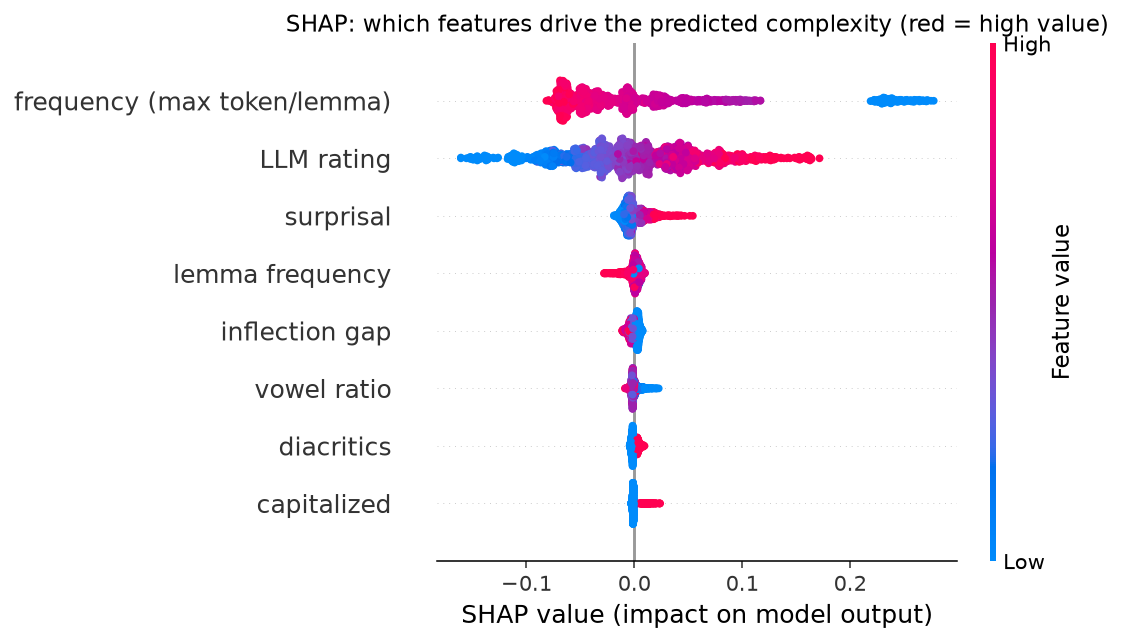
\includegraphics[width=\columnwidth]{beeswarm.png}
\caption{SHAP over named features (top 8 shown). Frequency dominates, then the LLM rating and surprisal. The
separate blue cluster on the frequency row is the group of very rare / out-of-vocabulary words, which push the
predicted complexity up --- the expected behavior. Red = high feature value.}
\label{fig:beeswarm}
\end{figure}

\begin{figure}[tbp]
\centering
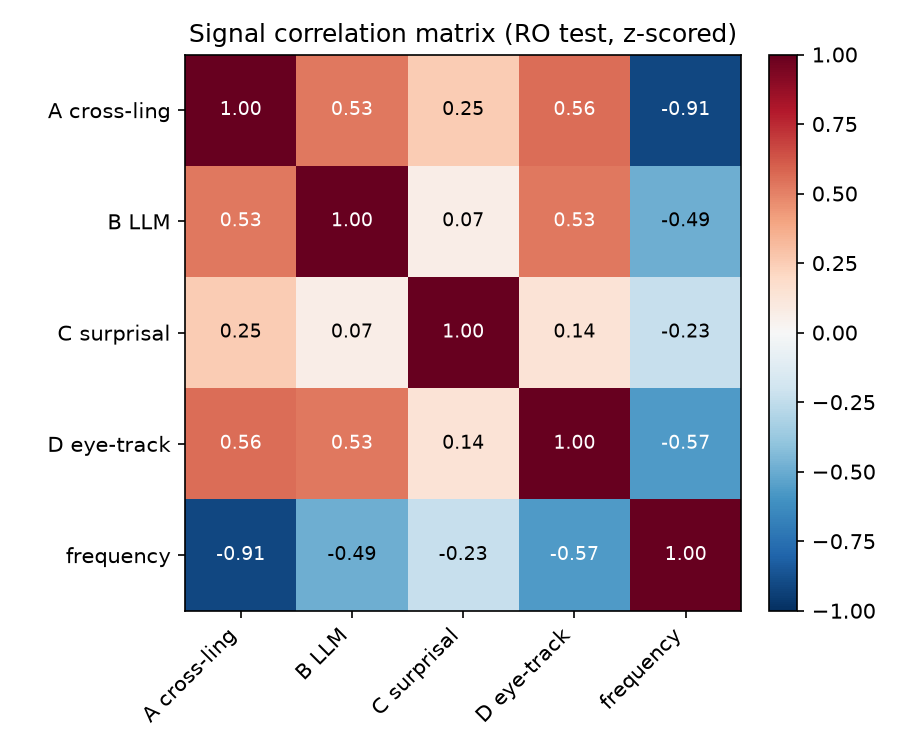
\includegraphics[width=\columnwidth]{fig_corr_matrix.png}
\caption{Correlation between the four signals and frequency on the Romanian test set. The rating (B) and surprisal
(C) are nearly independent; the cross-lingual signal (A) tracks frequency closely.}
\label{fig:corr}
\end{figure}

\subsection{Eye-tracking and an in-source check}
Eye-tracking helps because it captures something the text signals do not. The quick, first-glance measures (how
long the eye first rests on a word) mostly reflect how common the word is, which signal~A already knows. The slower
measures (re-reading a word, or looking back to it) reflect how hard the word is to fit into the sentence, and
these line up with surprisal \citep{gaze4nlp2025surprisal}. So eye-tracking mainly adds this ``hard to integrate in
context'' part on top of the other signals. As a separate check, the regressor sorts held-out English words into
easy, medium and hard groups cleanly (Figure~\ref{fig:confusion}).

\begin{figure}[tbp]
\centering
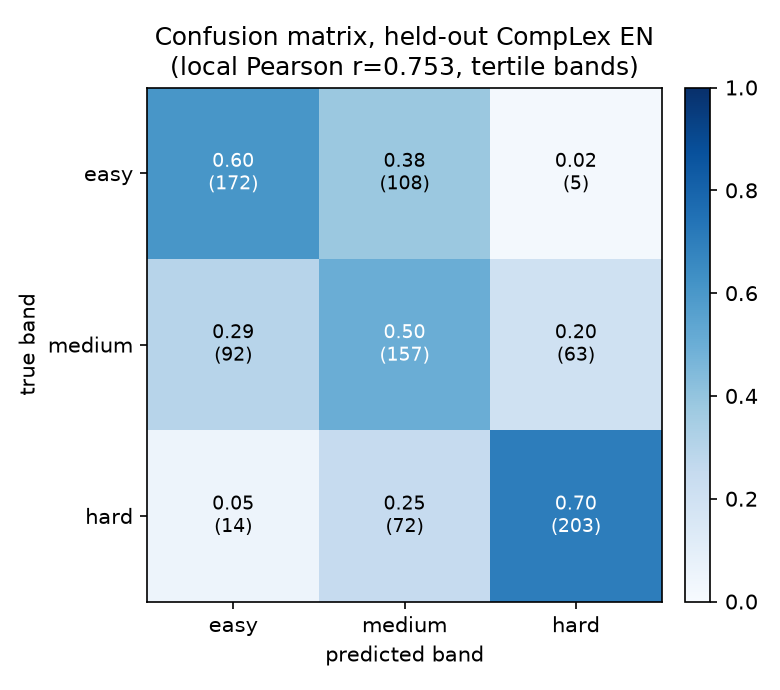
\includegraphics[width=0.8\columnwidth]{fig_confusion.png}
\caption{In-source check: on held-out English words, the regressor sorts complexity into easy/medium/hard bands
with a clearly diagonal confusion matrix.}
\label{fig:confusion}
\end{figure}

\begin{table}[tbp]
\centering\small
\begin{tabular}{lcc}
\toprule
\textbf{Configuration} & \textbf{Score} & \textbf{$\Delta$} \\
\midrule
Predict a constant (the mean) & 0.00 & --- \\
Surface features only (zero-shot RO) & 10.27 & +10.27 \\
\;+ eye-tracking (no external res.) & 41.76 & +31.49 \\
\;+ cross-lingual A + LLM B & 64.52 & +22.76 \\
\;+ surprisal C & 64.81 & +0.29 \\
\;+ lemma-frequency fix (in A) & 68.90 & +4.09 \\
\;+ eye-tracking PCA D & \textbf{69.74} & +0.84 \\
\bottomrule
\end{tabular}
\caption{Evaluation score, built one component at a time. $\Delta$ is the marginal contribution of each component.
Predicting one constant value for every word gives no correlation, hence a score of $0$. The best result without
external resources is $41.76$; the lemma-frequency fix is the largest single gain.}
\label{tab:ablation}
\end{table}

\begin{table}[tbp]
\centering\small
\begin{tabular}{lcc}
\toprule
\textbf{Signal} & \textbf{SHAP importance} & \textbf{weight} \\
\midrule
A cross-lingual & 0.061 & 44\% \\
B LLM rating & 0.034 & 29\% \\
D eye-tracking & 0.017 & 20\% \\
C surprisal & 0.006 & 6\% \\
\bottomrule
\end{tabular}
\caption{Per-signal SHAP importance and the weight each signal gets in the final average. The two orders agree;
SHAP describes the model, it does not choose the weights.}
\label{tab:signals}
\end{table}

\begin{table}[tbp]
\centering\small
\begin{tabular}{lc}
\toprule
\textbf{Eye-tracking metric} & \textbf{PC1 loading} \\
\midrule
Total fixation time (TFT) & 0.44 \\
Total fixation count (TFC) & 0.43 \\
First-pass reading time (FPRT) & 0.42 \\
First-pass fixation count (FPFC) & 0.39 \\
Re-reading time (RRT) & 0.35 \\
First-fixation duration (FFD) & 0.29 \\
Regression-path duration (RPD\_inc) & 0.28 \\
Incoming regressions (TRC\_in) & 0.13 \\
\bottomrule
\end{tabular}
\caption{Weight of each eye-tracking metric in the reading-effort score (loadings on PC1, which explains $62\%$ of
the variance). All loadings are positive: one ``more effort = more complex'' axis.}
\label{tab:pca}
\end{table}

\section{What Did Not Work}
\label{sec:negative}
Table~\ref{tab:fail} lists the main failures. Fine-tuning XLM-RoBERTa (in every form tried) did worse than leaving
it frozen: with no Romanian labels, fine-tuning over-fits the source language and breaks the multilingual alignment
the approach relies on. Several changes that looked good in the in-source check dropped on the public evaluation,
because the check measures transfer between English and Romance, not transfer to Romanian. Chain-of-thought and
few-shot prompting added noise rather than signal --- at this model size, chain-of-thought does not yet help
\citep{wei2022cot}. Rarity and a range of part-of-speech, named-entity and WordNet features also turned out to be
redundant with frequency.

\begin{table}[tbp]
\centering\small
\begin{tabular}{lcc}
\toprule
\textbf{Attempt} & \textbf{in-source} & \textbf{score} \\
\midrule
Frozen XLM-R (this work) & 0.515 & --- \\
Full fine-tune (best) & 0.461 & --- \\
LoRA (best) & 0.462 & --- \\
Encoder swap (e5) & 0.586 & 63.00 \\
Mid-layer embeddings & 0.556 & 64.49 \\
Lasso regressor & 0.569 & 64.28 \\
LLM few-shot prompt & --- & 63.31 \\
\bottomrule
\end{tabular}
\caption{Failed attempts. \emph{in-source} is the transfer correlation between English and Romance; the e5,
mid-layer and Lasso rows win there but drop on the public evaluation.}
\label{tab:fail}
\end{table}

\section{Conclusions}
\label{section:conclusions}
The lack of Romanian training data with complexity shaped the overall design: several independent signals are
built from outside resources and combined, instead of training a model that cannot be trained. The weights are
tuned against the public evaluation score, so some over-fitting to it is possible; the smooth tuning curves and the
in-source check argue the signals are real, and three final model variants relying on eye-tracking to different
degrees are kept as a hedge. Two conclusions stand out: a strong in-source score does not guarantee good transfer
to Romanian, and combining several transferred signals can perform well even without any labeled training data for
the task.

The code and data are available in this
\href{https://github.com/curs-ia-2026/ia-sahistii}{GitHub repository}.

\bibliographystyle{acl_natbib}
\bibliography{custom}

\end{document}
